\clearpage
\section{Installation Openhab}\label{sec:Openhab}
Openhab ist die Schnittstelle, welche in diesem Projekt die Geräte mit einender verknüpft. Die Opensource Software wird auf dem Raspberrypi 4 mit 2 GB RAM installiert und in Betrieb genommen. 

\subsection{Openhab Betriebssystem aufsetzen}
\begin{enumerate}
	\item Betriebsystem Download von der Offiziellen Openhab Webseite \cite{noauthor_download_nodate-1}, anschliessend Image auf Micro SD-Card mit Balena Etcher flashen.
   \item Auf SD-Card in Order "openhabian.conf" File mit Lokalen Wlan Namen "ssid" und Passwort "psk" erweitern.
   \item SD-Card auswerfen, Raspi mit SD-Card ausstatten und in Betrieb nehmen. Ein neuer Teilnehmer wird sichtbar im eigenen Netzwerk, Gerätenahme "openhab".
   \item Im Browser kann das Installierte Betriebssystem unter der IP Adresse und mit dem Port 8080 erreicht werden: http://192.168.137.51:8080/ Packet Standard Installieren. Dauert 20 min.
   \item Mit Konsole Openhabian, bearbeiten : \colorbox{lightgray}{sudo ssh openhabian@192.168.137.24}. \\
   Default Passwort "openhabian"
   \item Statische IP-Adresse vergeben: File dhcpcd.conf öffnen \colorbox{lightgray}{sudo nano /etc/dhcpcd.conf}. Interface eth0 zu wlan0 ändern 
   \begin{figure}[H]
   	\centering
   	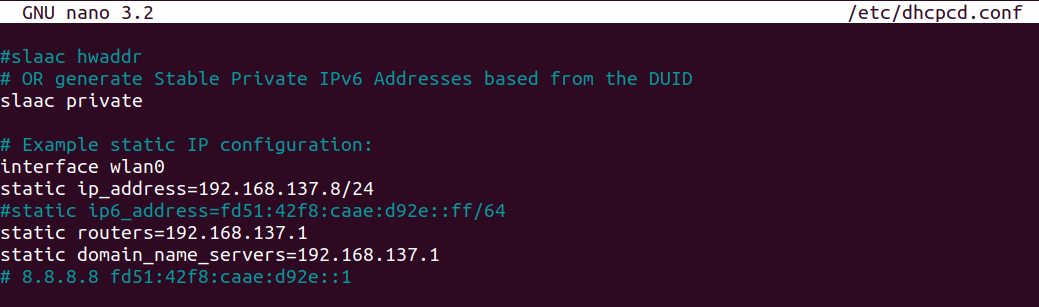
\includegraphics[width=0.9\textwidth]{graphics/dhcpcd.png}
   	\caption{File: dhcpcd.conf} 	
   	\label{pic: dhcpcd}
   \end{figure} 
\item Um Openhabian weiterhin mit Konsole zu erreichen müssen sich die Verschiedenen Geräten, Notebook und Raspi im gleichen IP-Adressraum befinden, eine Änderung kann mittels Adapteroptionen, Eigenschaften Internetprotokoll IPV4, folgende Adresse vergeben durchgeführt werden.

\item Um Konfigurationen mit Visual Studio Code zu Bearbeiten wird der Ordner openHab-conf in Netzlaufwerk vom Notebook verbunden. Eingabe Ordner: "\textbackslash \textbackslash 192.168.137.8 \textbackslash openHAB-conf" verbinden, mit andern Anmeldedaten anmelden Username:"openhabian", Passwort: "openhabian" wählen.

\item Visual Studio Code öffnen Ordner öffnen openHab-conf wählen. In Einstellungen, Erweiterungen, OpenHab Configuration, Host in "settings.json" bearbeiten wählen. \\
\colorbox{lightgray}{openhab.host: "192.168.137.8",
	"git.autofetch": true} eingeben.
   
   
 \end{enumerate}